\documentclass{article}
\usepackage[T1]{fontenc}
\usepackage{amssymb}
\usepackage{listings}
\usepackage[utf8x]{inputenc}
\usepackage{amsmath,amssymb}
\usepackage{pdfpages}
\usepackage[russian,english]{babel}
\lstset{
    language=Octave,
    frame=single,
    inputencoding=utf8x,
    extendedchars=\true,
    texcl=\false,
    commentstyle={}
}
\usepackage[a4paper,top=1cm,bottom=2cm,left=1.5cm,right=1cm,marginparwidth=1.75cm]{geometry}

\makeatletter
\def\@seccntformat#1{
  \expandafter\ifx\csname c@#1\endcsname\c@section\else
  \csname the#1\endcsname\quad
  \fi}
\makeatother

\begin{document}

\selectlanguage{russian}
\title{Лабораторная работа 4, ТВМС}
\author{
	Бочарников Андрей, M3238\\
	Ковешников Глеб, M3238\\
	Шишкин Алексей, M3238
}
\maketitle

\begin{quote}
\selectlanguage{russian}
\section{Формулировка}
	Для случайной величины, распределенной по нормальному закону с параметрами ($a$,$\sigma^2$), выполнить следующие действия:\\\\
	1. Задать параметры распределения $X \thicksim N(a, \sigma^2)$.\\
	2. Построить выборку генеральной совокупности $X$.\\
	3. Построить график гистограммы.\\
	4. Проверить гипотезу о виде распределения по критерию хи-квадрат.\\
	Аналогично для $X \thicksim U(a, b)$ - равномерно распределенной на $[a, b]$ случайной величины.
\section{Входные данные}
        \begin{itemize}
            \item Выборка генеральной совокупности: $n = 10^5$
            \item TODO.
        \end{itemize}
\section{Программа 1}
	Нормальное распределение.
\subsection{Исходный код}
	\lstinputlisting{task1.m}
\subsection{График}
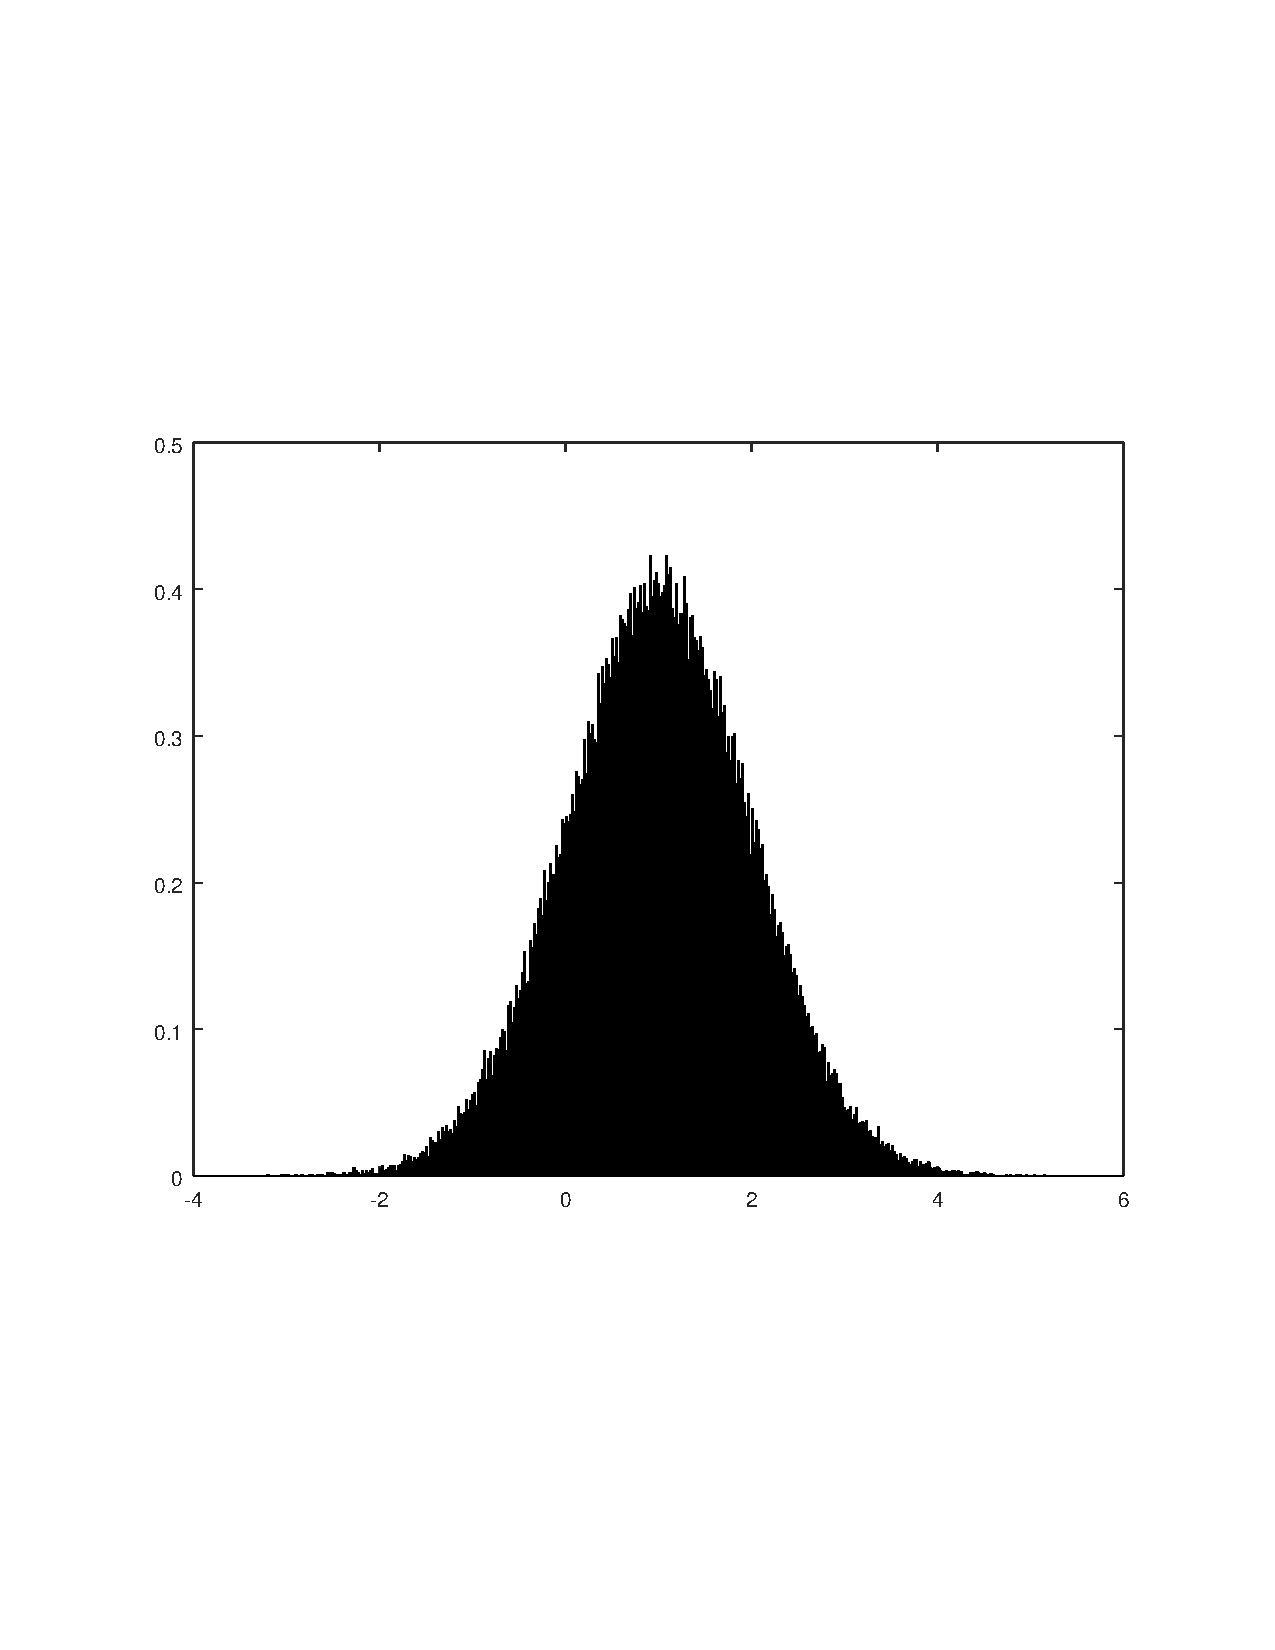
\includepdf[width=\textwidth]{normcdf.pdf}
\section{Программа 2}
	Равномерное распределение.
\subsection{Исходный код}
	\lstinputlisting{task2.m}
\subsection{График}
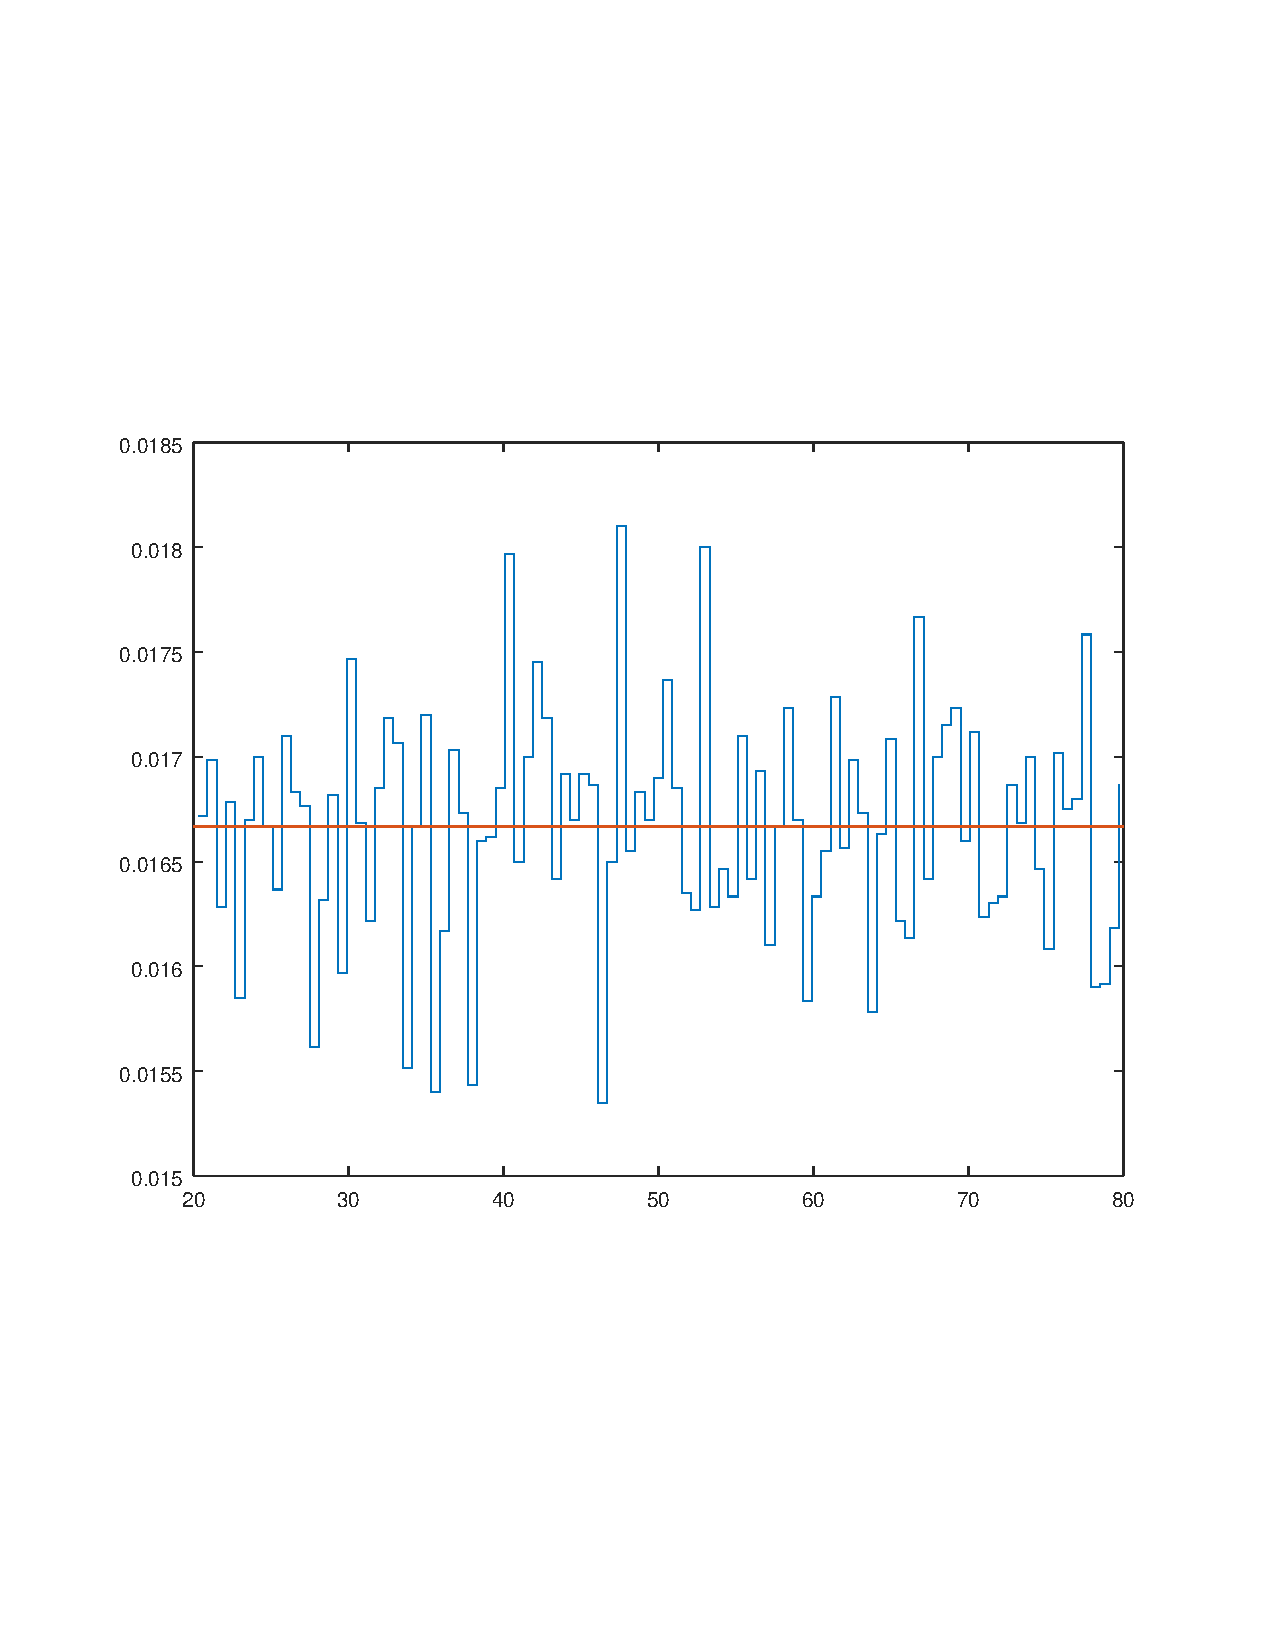
\includepdf[width=\textwidth]{unicdf.pdf}
\section{Вывод}
	TODO.
\end{quote}
\end{document}
